\documentclass{article}
\usepackage{graphicx} % Required for inserting images
\usepackage{geometry}
\usepackage{circuitikz}
\usepackage{siunitx}
\usepackage{CJKutf8}
\usepackage{amsmath}
\usepackage{amssymb}
\usepackage{caption}
\usepackage{float}
\usepackage{subcaption}
\geometry{top=5mm, left=30mm, a4paper}

\title{Oscillators and Signal Generators Report}
\author{梁程捷 (B11901136), 吳奕娃 (B11901080)}
\date{}


\begin{document}
\begin{CJK*}{UTF8}{bkai}

\maketitle

\section*{Generation of Triangular and Square Waveforms}

\begin{figure}[h]
    \begin{center}
        \begin{subfigure}[b]{0.55\textwidth}
            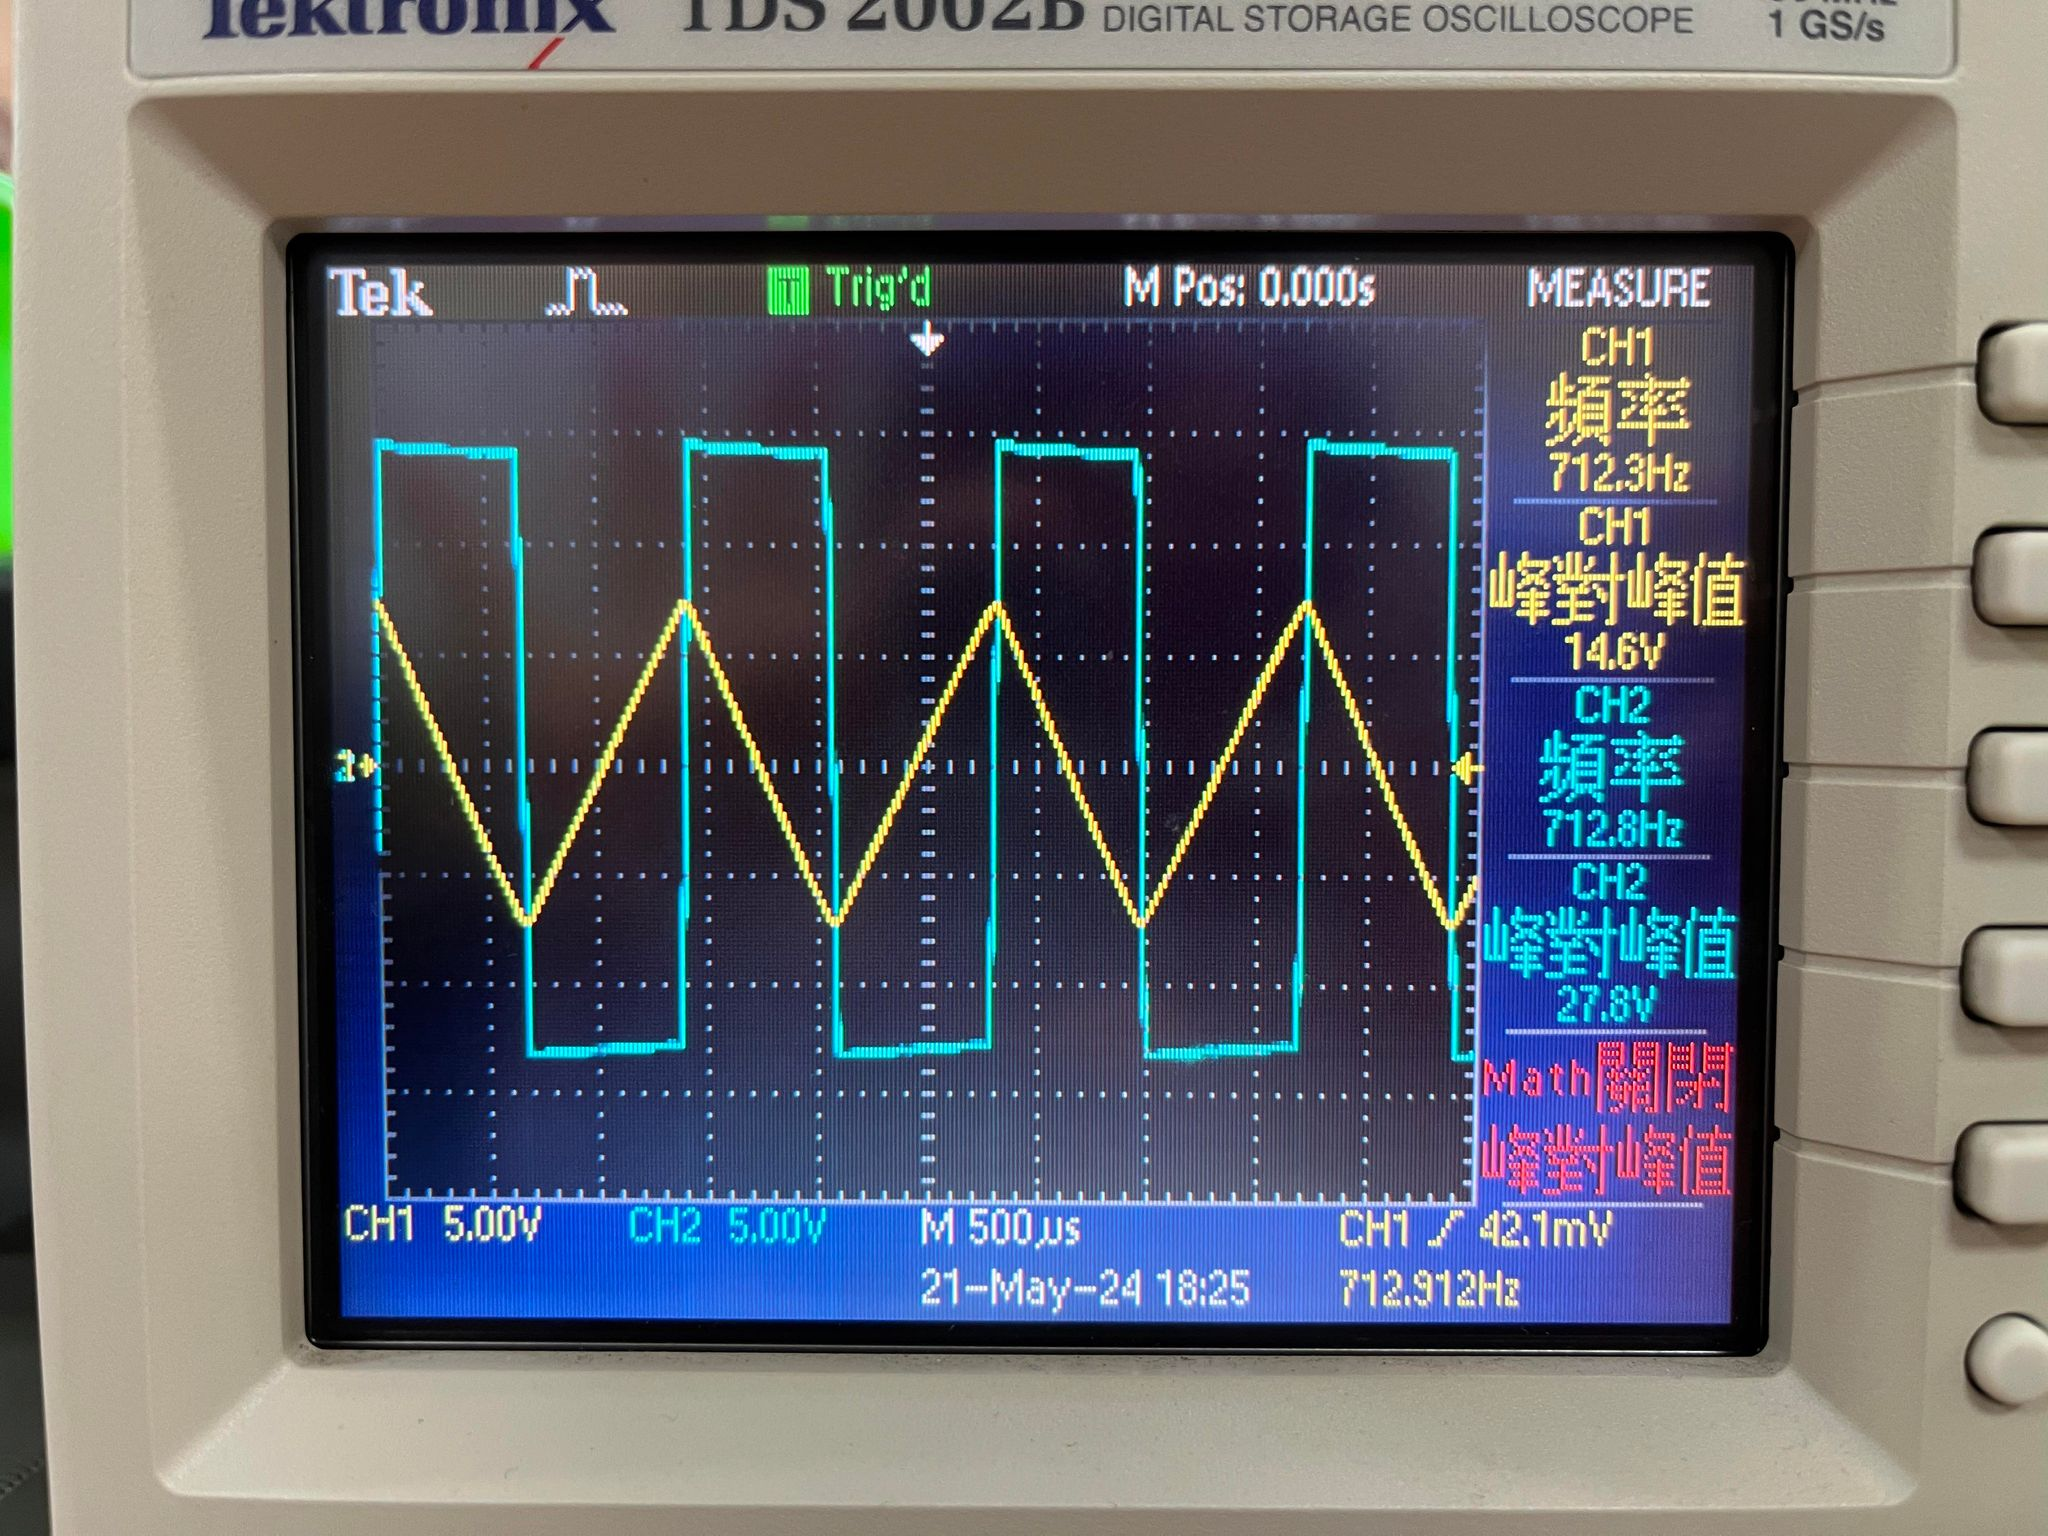
\includegraphics[width=\textwidth]{square_wave_gen.jpg}
            \caption*{Output waveforms of CH1 and CH2 in Y-t mode}
        \end{subfigure}
    \end{center}
\end{figure}
From the figure, the output frequency is \textbf{712.3 \unit{\hertz}} 

\section*{Conclusion}
The generation of square wave is from the output of non-inverting bistable circuit, and the triangular wave is from the output of
the square wave through an integrator.

\section*{Reflections}
\subsection*{梁程捷}
這次實驗感覺很有趣,電路也不會太困難,也理論課對上了,在沒有外接function generator的情況下就自己產生了波形。

\subsection*{吳奕娃}
我覺得這次的實驗相對簡單,第一次嘗試就成功了,這個電路在沒有接示波器的情況下產生方波和三角波,讓我覺得很有趣。
    
\end{CJK*}
\end{document}